\chapter{Specifications}\label{specifications}

\section{Functional Description}\label{functional-description}

The
Roa Logic AHB-Lite APB4 Bridge is a highly configurable, fully
parameterized soft IP interconnect bridge between the \emph{AMBA 3
AHB-Lite v1.0} and \emph{AMBA APB v2.0} bus protocols.

These protocols are commonly referred to as AHB-Lite and APB4
respectively -- these terms will be used throughout this datasheet. All
signals defined in the AHB-Lite and APB4 specifications are fully
supported.

The IP contains 2 interfaces; an AHB-Lite Slave Interface and an APB4
Master Interface. Transactions received on the AHB-Lite Slave Interface
are translated into APB4 transactions on the APB4 Master Interface. The
IP automatically generates APB4 burst transactions if the APB4 data
width is less than the AHB-Lite data width.

\begin{figure}[tbh]
	\centering
	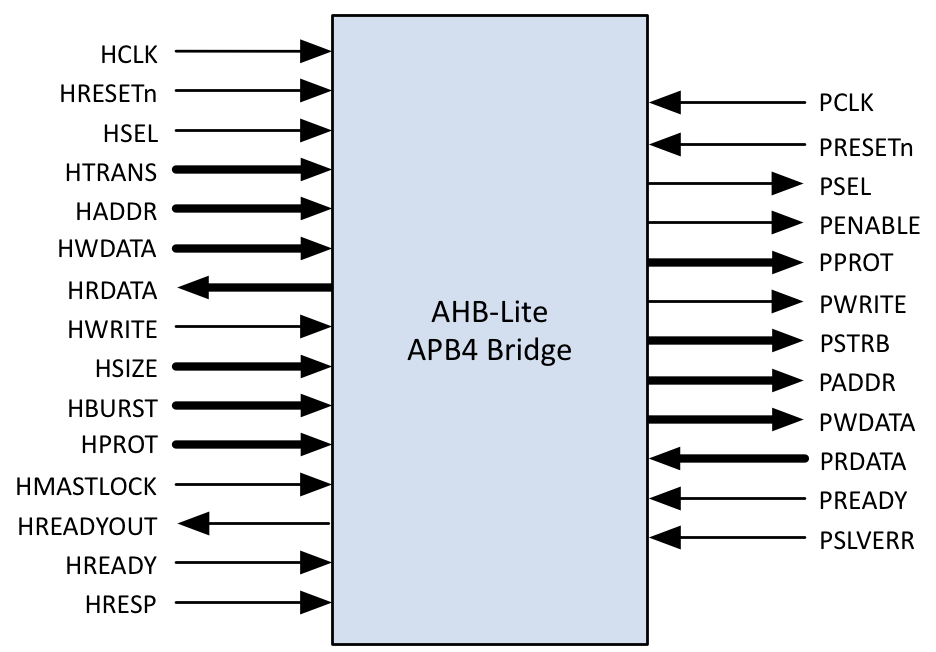
\includegraphics{assets/img/apb4-bridge-sig.png}
	\caption{Bridge Signaling}
	\label{fig:apb4-bridge-sig}
\end{figure}

Each interface can operate on a separate clock domain and the IP
automatically handles all cross clock domain synchronization
requirements.

\begin{longtable}[]{@{}|rp{12cm}@{}}
	\textbf{Notes:} & \tabularnewline
	\endhead
	1. & The APB4 Interface clock frequency must be less than or equal 
	to the AHB-Lite interface clock frequency\\
	2. & The APB4 Interface data width must be less than or equal to 
	the data width of the AHB-Lite interface\\
	3. & AHB-Lite and APB4 Interface data widths must be an integer 
	multiple of bytes.\\
\end{longtable}

	
\section{AHB-Lite Interface}\label{ahb-lite-interface}

An AHB-Lite Bus Master connects to the AHB interface of the AHB-Lite
APB4 Bridge. The AHB interface is implemented as a regular AHB-Lite
Slave Interface, supporting all signals in the \emph{AMBA 3 AHB-Lite
v1.0} protocol specification

\section{APB4 Interface}\label{apb4-interface}

An APB4 Bus Slave connects to the APB interface of the Bridge IP. The
APB port is implemented as a regular APB4 Master Interface supporting
all signals of the \emph{AMBA APB v2.0} protocol specification. This
allows a single APB4 Peripheral to be connected directly to the
Interface without further logic requirements.

Multiple peripherals can share the APB4 Interface through appropriate
decoding and multiplexing of the interface signals. Roa Logic provides
an additional APB4 Multiplexer IP to implement this capability.

\begin{figure}[tbh]
	\centering
	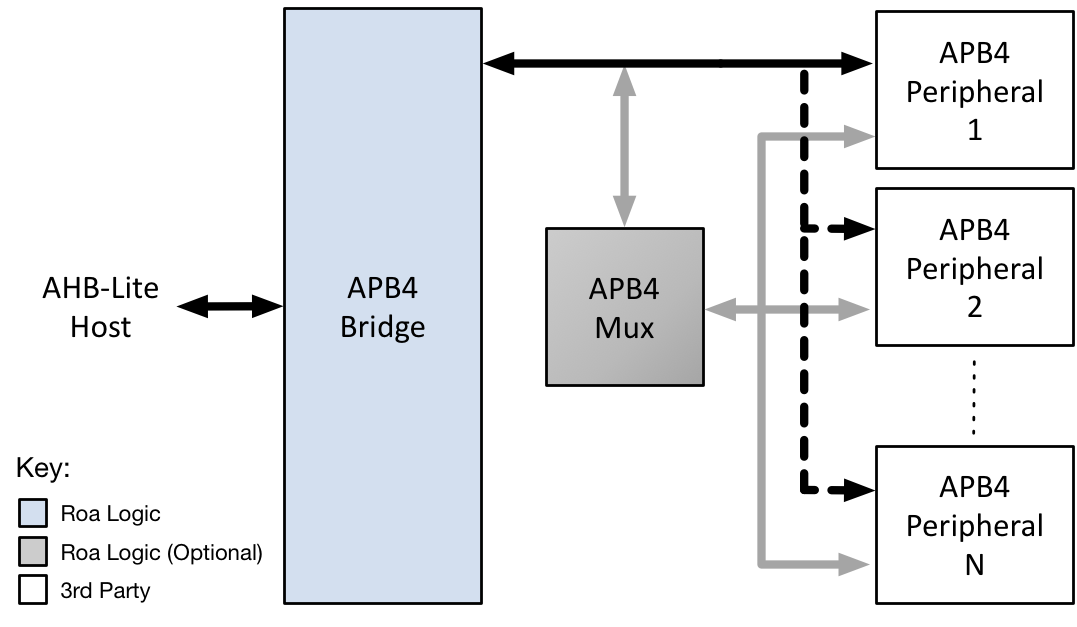
\includegraphics{assets/img/apb4-bridge-sys.png}
	\caption{APB4 Multiplexing Peripherals}
	\label{fig:apb4-bridge-sys2}
\end{figure}